\section{The Earth's magnetic field}
The Earth's magnetic field dictates the morphology and natural coordinate systems used in studying the near-Earth space environment. Here we discuss three models of the Earth's magnetic field, with increasing complexity and realism.
\subsection{Models of the magnetic field}
\paragraph{Dipole}
\label{section:dipole_model}
To first order, the Earth's magnetic field can be approximated as a dipole, with origin at the Earth's center, and a tilt of $\approx 11^\circ$ from the axis of rotation. The dipole model, sometimes referred to as the ``centered dipole'' or ``tilted dipole'', is reasonably accurate for midlatitude field measurements over the continental United States, but can deviate significantly from the true field elsewhere. Similarly, the dipole field model is reasonably accurate for middle latitudes, below $\approx$ 10 Earth radii, but becomes increasingly inaccurate at higher latitudes, and at larger distances from the Earth, where the Earth's internal field is no longer dominant.

The dipole model, however, excels in its simplicity -- the dipole magnetic field can be completely described in a closed form, and can be computed rapidly and reliably.

The magnetic dipole potential is given by:
\begin{equation}
\psi_{dip} = B_0\big(\frac{R_e}{r}\big)^2\cos\theta
\end{equation}

The individual components of the magnetic field are given by the negative gradient of the scalar potential:

\begin{eqnarray}
& \vec{B} = -\nabla \psi \\
& B_r = -2 B_0\big(\frac{R_e}{r}\big)^3\cos\theta \\
& B_{\theta} = -B_0\big(\frac{R_e}{r}\big)^3 \sin\theta \\ 
& B_\phi = 0
\end{eqnarray}

Within this work we use $B_0 = 31.5$ $\mu$T and $R_e=6371$ km.

A single fieldline, determined by integrating the direction of the field vector, can be described by it's \emph{L-shell} -- the fieldline's altitude, in units of Earth radii, measured at the equator. 

For the dipole field, the radius of a field line at any latitude is related by:
\begin{equation}
R(\lambda) = R_e L \cos^2 \lambda
\end{equation}


The dipole field can then be used as an orthogonal coordinate system, with any location being specified by a latitude, longitude, and L-shell \citep{McIlwain1961}. 

Within the plasmasphere, the dipole model works well. However, closer to the Earth's surface the model becomes increasingly inaccurate, necessitating a higher-order model.
\paragraph{IGRF}
The International Geomagnetic Reference Field (IGRF) is a 13th-order spherical expansion model, with coefficients updated every few years based on terrestrial measurements \citep{Thebault2015}. Within this work we use the IGRF-12 model as a realistic representation of the Earth's internal magnetic field.

IGRF is quick and simple to calculate at any given location, and is much closer to reality than a simple dipole field. However, due to the added complexity, there are not closed-form expressions for field line trajectories or L-shells, which can make dealing with IGRF (and any higher-order model) more cumbersome.

Figure \ref{fig:Lshell_example} contrasts lines of constant L-shell between the dipole and IGRF models.

\paragraph{Tsyganenko Corrections}
The dipole and IGRF models represent the Earth's internally-generated magnetic field. However, as one moves further away from the Earth ($L > \sim 8$), the Earth's internal field becomes less dominant, and external fields, namely forcing from the solar wind, cannot be ignored. The total field present in the space environment is the sum of both internal and external contributions.

Numerous models of the external field exist; within this work we consider the T05 external field model \citep{Tsyganenko2005}. The external field model exhibits seasonal and daily variation. However, for fieldlines below L $\approx$ 6, the external field effects can be ignored. 

Figure \ref{fig:fieldline_example} contrasts the dipole, IGRF, and T05-corrected models in the meridional plane; Figure \ref{fig:Lshell_example} illustrates the deviation in fieldline contours along the Earth's surface between the dipole and IGRF models.

\begin{figure}[t]
\begin{center}
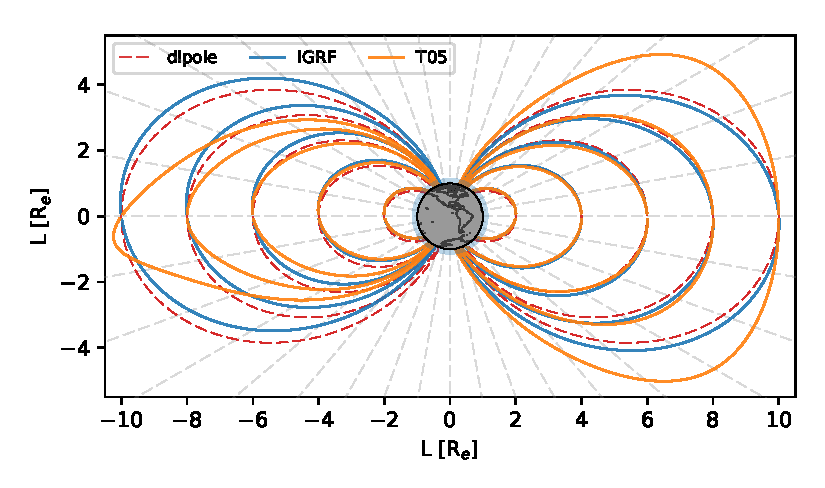
\includegraphics{figures/fieldline_models.pdf}
\end{center}

\caption[Magnetic field models]{Three different magnetic field models, shown in the meridional plane, in geomagnetic coordinates: the tilted dipole, the IGRF model, and the Tsyganenko-Corrected IGRF model. Solar wind is incident on the right side.}
\label{fig:fieldline_example}
\end{figure}
\begin{figure}
\begin{center}
	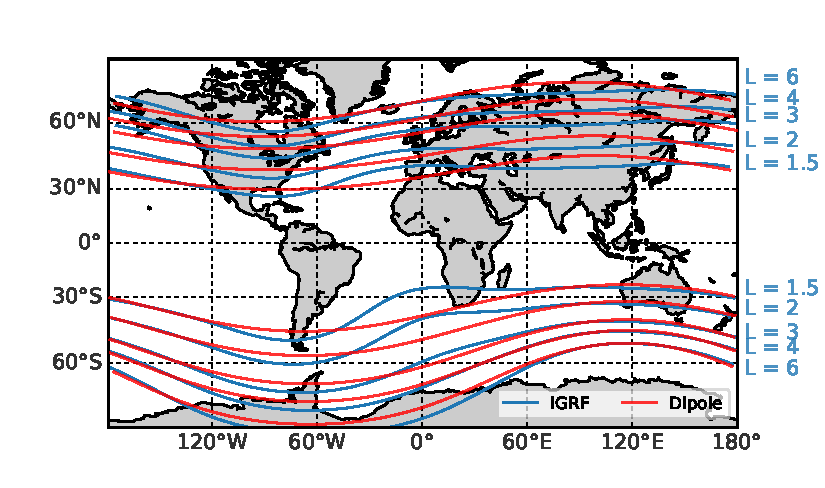
\includegraphics{figures/Lshell_contours.pdf}
\end{center}
\caption[L-shell contours on the Earth's surface]{Fieldline contours along the Earth's surface, shown for the dipole and IGRF models.}
\label{fig:Lshell_example}
\end{figure}

